\documentclass[aspectratio=1610,onlymath]{beamer}
% \documentclass[aspectratio=1610,onlymath,handout]{beamer}

\input{macros-lecture}
% Common notation

\usepackage{amsmath,amssymb,amsfonts}
\usepackage{xspace}

\newcommand{\lectureurl}{https://iccl.inf.tu-dresden.de/web/FS2023}

\DeclareMathAlphabet{\mathsc}{OT1}{cmr}{m}{sc} % Let's have \mathsc since the slide style has no working \textsc

% Dual of "phantom": make a text that is visible but intangible
\newcommand{\ghost}[1]{\raisebox{0pt}[0pt][0pt]{\makebox[0pt][l]{#1}}}

\newcommand{\tuple}[1]{\langle{#1}\rangle}
\newcommand{\defeq}{\mathrel{:=}}

%%% Annotation %%%

\usepackage{color}
\newcommand{\todo}[1]{{\tiny\color{red}\textbf{TODO: #1}}}



%%% Old macros below; move when needed

\newcommand{\blank}{\text{\textvisiblespace}} % empty tape cell for TM

% table syntax
\newcommand{\dom}{\textbf{dom}}
\newcommand{\adom}{\textbf{adom}}
\newcommand{\dbconst}[1]{\texttt{"#1"}}
\newcommand{\pred}[1]{\textsf{#1}}
\newcommand{\foquery}[2]{#2[#1]}
\newcommand{\ground}[1]{\textsf{ground}(#1)}
% \newcommand{\foquery}[2]{\{#1\mid #2\}} %% Notation as used in Alice Book
% \newcommand{\foquery}[2]{\tuple{#1\mid #2}}

\newcommand{\quantor}{\mathord{\reflectbox{$\text{\sf{Q}}$}}} % the generic quantor

% logic syntax
\newcommand{\Inter}{\mathcal{I}} %used to denote an interpretation
\newcommand{\Jnter}{\mathcal{J}} %used to denote another interpretation
\newcommand{\Knter}{\mathcal{K}} %used to denote yet another interpretation
\newcommand{\Zuweisung}{\mathcal{Z}} %used to denote a variable assignment

% query languages
\newcommand{\qlang}[1]{{\sf #1}} % Font for query languages
\newcommand{\qmaps}[1]{\textbf{QM}({\sf #1})} % Set of query mappings for a query language

%%% Complexities %%%

\hyphenation{Exp-Time} % prevent "Ex-PTime" (see, e.g. Tobies'01, Glimm'07 ;-)
\hyphenation{NExp-Time} % better that than something else

% \newcommand{\complclass}[1]{{\sc #1}\xspace} % font for complexity classes
\newcommand{\complclass}[1]{\ensuremath{\mathsc{#1}}\xspace} % font for complexity classes

\newcommand{\ACzero}{\complclass{AC$_0$}}
\newcommand{\LogSpace}{\complclass{L}}
\newcommand{\NLogSpace}{\complclass{NL}}
\newcommand{\PTime}{\complclass{P}}
\newcommand{\NP}{\complclass{NP}}
\newcommand{\coNP}{\complclass{coNP}}
\newcommand{\PH}{\complclass{PH}}
\newcommand{\PSpace}{\complclass{PSpace}}
\newcommand{\NPSpace}{\complclass{NPSpace}}
\newcommand{\ExpTime}{\complclass{ExpTime}}
\newcommand{\NExpTime}{\complclass{NExpTime}}
\newcommand{\ExpSpace}{\complclass{ExpSpace}}
\newcommand{\TwoExpTime}{\complclass{2ExpTime}}
\newcommand{\NTwoExpTime}{\complclass{N2ExpTime}}
\newcommand{\ThreeExpTime}{\complclass{3ExpTime}}
\newcommand{\kExpTime}[1]{\complclass{#1ExpTime}}
\newcommand{\kExpSpace}[1]{\complclass{#1ExpSpace}}


\usetikzlibrary{shapes}

\defineTitle{16}{Kellerautomaten \& CFGs}{4. Dezember 2023}

\begin{document}

\maketitle

% \sectionSlide{Vorschau}
% 
% 
% \begin{frame}\frametitle{Plan}
% 
% \begin{itemize}
% \item \alert{Grammatiken}
% \item \alert{Reguläre Sprachen}
% \begin{itemize}
% \item DFA und NFA
% \item Umformungen, Abschlusseigenschaften, Minimalisierung
% \item Pumping Lemma
% \end{itemize}
% \item \alert{Kontextfreie Sprachen}
% \begin{itemize}
% \item Wortproblem (CYK)
% \item Pumping Lemma
% \item Kellerautomaten
% \end{itemize}\pause
% \item \alert{Typ 1 und Typ 0}
% \begin{itemize}
% \item Turingmaschinen
% \item (Un)Entscheidbarkeit
% \end{itemize}
% \item \alert{Aussagenlogik}
% \begin{itemize}
% \item Syntax und Semantik
% \item Algorithmen zum logischen Schließen
% \item Die Komplexitätsklasse NP
% \end{itemize}
% \end{itemize}
% 
% \end{frame}

\sectionSlideNoHandout{Rückblick}

\begin{frame}\frametitle{Kellerautomat = NFA + Stapelspeicher}

\narrowcentering{%
\begin{tikzpicture}[
	scale=0.50,
	decoration=penciline, decorate
]
% \path[use as bounding box] (-3.2,0) rectangle (3.5,-5); % add "draw" to see it
% \draw[help lines] (0,0) grid (5,5);
\pgfmathsetseed{5712}
%
\node (inlabel) [circle,draw=none,inner sep=1pt] at (2,0.5) {\alert{Eingabewort}};
\draw[fill=none,decorate,line width=0.3mm] (0,0) -- (6,0);
\draw[fill=none,decorate,line width=0.3mm] (0,-1) -- (6,-1);
\foreach \x in {0,...,4} {
	\draw[fill=none,decorate,line width=0.3mm] (\x,0) -- (\x,-0.9);
	\node (s\x) [circle,draw=none,inner sep=1pt] at (\x+0.5,-0.5) {\ifthenelse{\x<4}{\Sterm{a}}{\Sterm{b}}};
}
\draw[fill=none,decorate,line width=0.3mm] (5,0) -- (5,-0.9);
\node (dots) [circle,draw=none,inner sep=1pt] at (5.8,-0.5) {$\cdots$};

\draw[fill=none,decorate,line width=0.3mm]
	(2,-3) -- (6,-3) -- (6,-7) -- (2,-7) -- cycle;
\node (falabel) [circle,draw=none,inner sep=1pt,align=left] at (4,-5) {Endliche\\Steuerung};
\draw[fill=none,decorate,line width=0.4mm,darkblue,->]
	(4,-3) -- (4,-2) -- (1.5,-2) -> (1.5,-1);

\node[rectangle,align=center,draw,line width=0.3mm,decorate, minimum width=8mm, minimum height=8mm] (state) at (8, -6) {$q$};
\draw[fill=none,decorate,line width=0.4mm,darkblue,->]
	(6,-6) -> (state.180);
\node (qlabel) [circle,draw=none,inner sep=1pt] at (11.5,-6) {\footnotesize\alert{Zustandsvariable}};

% \node[cloud, cloud puffs=15.7, cloud ignores aspect, minimum width=4cm, minimum height=1cm, align=center, draw,line width=0.3mm] (memory) at (11, -1) {\alert{zusätzlicher}\\\alert{Speicher}};

\draw[fill=none,decorate,line width=0.3mm] (9,0) -- (9,-4);
\draw[fill=none,decorate,line width=0.3mm] (10,0) -- (10,-4);
\draw[fill=none,decorate,line width=0.3mm] (8.5,-4) -- (10.5,-4);
\foreach \y in {0,...,-3} {
	\draw[fill=none,decorate,line width=0.3mm] (9,\y) -- (10,\y);
	\node (k\y) [circle,draw=none,inner sep=1pt] at (9.5,\y-0.5) {\ifthenelse{\y<-1}{\Snterm{A}}{\Snterm{B}}};
}
\draw[fill=none,decorate,line width=0.4mm,darkblue,->]
	(6,-3.5) -- (7.5,-3.5) -- (7.5,-0.5) -> (9,-0.5);
\node (stacklabel) [circle,draw=none,inner sep=1pt] at (11.5,-2.5) {\alert{Keller}};
\end{tikzpicture}}

Eine mögliche \redalert{Konfiguration} des PDA während der Erkennung ist gegeben durch
den Zustand $q\in Q$, den Inhalt des Kellers $\gamma\in\Gamma^*$ und das noch zu lesende Restwort $w\in\Sigma^*$.

% Wir können auch für PDAs eine Übergangsfunktion definieren:

\end{frame}

\begin{frame}\frametitle{Kellerautomaten (PDAs)}

Beispiel eines PDA für $\{\Sterm{a}^i\Sterm{b}^i\mid i\geq 0\}$:
\bigskip

\narrowcentering{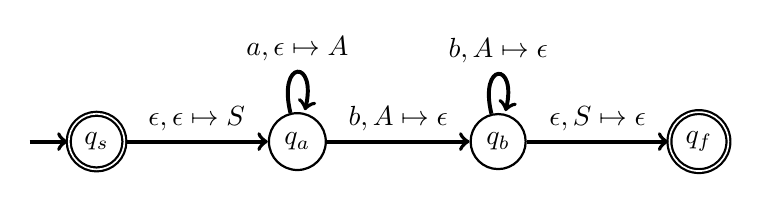
\begin{tikzpicture}[xscale=0.85,baseline={([yshift=-2ex]current bounding box.north)}]
% \draw[help lines] (0,0) grid (7,2);
\node (s) [circle,draw=black,thick,double] at (0,0) {$q_s$};
\node (a) [circle,draw=black,thick] at (3,0) {$q_a$};
\node (b) [circle,draw=black,thick] at (6,0) {$q_b$};
\node (f) [circle,draw=black,thick,double] at (9,0) {$q_f$};
%
\path[->,line width=0.5mm](-1,0) edge (s);
\path[->,line width=0.5mm](s) edge node[above] {$\epsilon,\epsilon\mapsto\Snterm{S}$} (a);
\path[->,line width=0.5mm](a) edge [loop above] node[above] {$\Sterm{a},\epsilon\mapsto\Snterm{A}$} (a);
\path[->,line width=0.5mm](a) edge node[above] {$\Sterm{b},\Snterm{A}\mapsto\epsilon$} (b);
\path[->,line width=0.5mm](b) edge [loop above] node[above] {$\Sterm{b},\Snterm{A}\mapsto\epsilon$} (b);
\path[->,line width=0.5mm](b) edge node[above] {$\epsilon,\Snterm{S}\mapsto\epsilon$} (f);
\end{tikzpicture}}\bigskip
% 
% Zur Vereinfachung der folgenden Definition schreiben wir $\Sigma_\epsilon$ für $\Sigma\cup\{\epsilon\}$ (und analog für $\Gamma_\epsilon$).\bigskip

\defbox{Ein \redalert{Kellerautomat} (international: "`\alert{PDA}"'/"`\alert{Pushdown Automaton}"') 
\Smach{M} ist ein Tupel $\Smach{M}=\tuple{Q,\Sigma,\Gamma,\delta,Q_0,F}$ mit
Zustandsmenge $Q$, Eingabealphabet $\Sigma$, Kelleralphabet $\Gamma$, Startzuständen $Q_0$, Endzuständen $F$
und Übergangsfunktion $\delta$:\\[1ex]
\narrowcentering{$Q\times\Sigma_\epsilon\times\Gamma_\epsilon \to 2^{Q\times\Gamma_\epsilon}$}\\[1ex]
wobei $\Sigma_\epsilon=\Sigma\cup\{\epsilon\}$ und $\Gamma_\epsilon=\Gamma\cup\{\epsilon\}$.
}

\end{frame}

\sectionSlide{Ausdrucksstärke von PDAs}

\begin{frame}\frametitle{Ausdrucksstärke von PDAs}

Man kann nun formal untersuchen, welche Sprachen durch PDAs akzeptiert werden können.
Wir erhalten das erhoffte Resultat:\medskip

\theobox{\emph{Satz:} Eine Sprache ist genau dann kontextfrei wenn sie von einem PDA akzeptiert wird.}\bigskip
% \theobox{Satz: Eine Sprache $\Slang{L}$ ist kontextfrei genau dann wenn es einen PDA $\Smach{M}$ mit 
% $\Slang{L}(\Smach{M})=\Slang{L}$ gibt.}\pause\bigskip

Der Beweis erfolgt in zwei Schritten:
\begin{enumerate}[(1)]
\item Umwandlung Typ-2-Grammatik $\leadsto$ PDA
\item Umwandlung PDA $\leadsto$ Typ-2-Grammatik
\end{enumerate}

\end{frame}


\begin{frame}[t]\frametitle{PDA $\leadsto$ Grammatik}

\theobox{\emph{Satz:} Für jeden PDA $\Smach{P}$ gibt es eine kontextfreie Grammatik $G_{\Smach{P}}$, so dass \ghost{$\Slang{L}(\Smach{P})=\Slang{L}(G_{\Smach{P}})$.}}\pause\bigskip

\emph{Beweisidee:}
Für jedes Paar von Zuständen $q$ und $r$ betrachten wir die Sprache
$\Slangsub{L}{q,r}$, die durch $\Smach{P}$ akzeptiert wird, wenn man mit leerem Keller in Zustand $q$ beginnt
und in Zustand $r$ \alert{mit leerem Keller} endet, d.h.
\[ w\in \Slangsub{L}{q,r} \quad\text{ genau dann wenn }\quad \tuple{q,w,\epsilon}\vdash^* \tuple{r,\epsilon,\epsilon}\]

\begin{itemize}
\item $\Slangsub{L}{q,r}$ wird in der Grammatik durch eine Variable $\Sntermsub{V}{q,r}$ dargestellt
\item Wir modifizieren $\Smach{P}$, so dass
\begin{itemize}
\item $\Smach{P}$ genau einen Startzustand $q_0$ und genau einen Endzustand $q_f$ hat
\item der Keller vor Erreichen von $q_f$ geleert werden muss
\end{itemize}
$\leadsto$ Die gesuchte Sprache $\Slang{L}(\Smach{P})$ ist genau $\Slangsub{L}{$q_0,q_f$}$
\end{itemize}

\end{frame}

\def\stackColA{darkred}
\def\stackColB{darkblue}
\def\stackColC{strongyellow}
\def\myRandomSeed{1851}

\newcommand{\drawStack}[4]{
\pgfmathsetseed{\myRandomSeed}
\foreach \i in {0,...,#1} {
	\ifthenelse{\i>0}{

	\pgfmathsetmacro\rnum{\i*random(17)}
	\pgfmathparse{(#4>0)?1:0}
	\ifthenelse{\pgfmathresult>0 \AND \i=#1 } {
		\pgfmathsetmacro\rnum{\rnum+#4)}
	}{}
	\pgfmathsetmacro\k{mod(\rnum,4)*33)}
	
	\pgfmathsetmacro\ir{random(4)}
	\pgfmathparse{(\ir>2)?1:0}
	\ifthenelse{\pgfmathresult=0}
	{
		\draw[fill=\stackColA!\k!\stackColC,line width=0.1mm] (#2,\l * #3 + \l * \i - \l) -- (#2+\l,\l * #3 + \l * \i - \l) -- (#2+\l,\l * #3 + \l * \i) -- (#2,\l * #3 + \l * \i) -- cycle;
	}{
		\draw[fill=\stackColB!\k!\stackColC,line width=0.1mm] (#2,\l * #3 + \l * \i - \l) -- (#2+\l,\l * #3 + \l * \i - \l) -- (#2+\l,\l * #3 + \l * \i) -- (#2,\l * #3 + \l * \i) -- cycle;
	}}{}
}
}

% \newcommand{\drawStair}[4]{
% 	\xdef\h{0}
% 	\xdef\nextinc{1}
% 
% 	\foreach \j in {1,...,#1} {
% 		\foreach \t in {1,...,\j} {
% 			\pgfmathsetmacro\r{random(4)} % unused, just advance random generator, which drawStack resets
% 		}
% 
% 		\ifthenelse{\nextinc=0}{
% 		}{
% 			\pgfmathparse{\h+1}
% 			\xdef\h{\pgfmathresult}
% 		}
% 		
% 		\pgfmathsetmacro\ir{random(4)}
% 		\pgfmathparse{(\ir>1)?1:0}
% 		\ifthenelse{\pgfmathresult=0}{
% 			\xdef\nextinc{0}
% 			\pgfmathsetmacro\randomtop{\j}
% 		}{
% 			\xdef\nextinc{1}
% 			\pgfmathsetmacro\randomtop{0}
% 		}
% 
% 		\pgfmathsetmacro\x{(#3+\j)*(\l+\xgap)}
% 		\drawStack{\h}{\x}{#4}{\randomtop}
% 	}
% }
% \newcommand{\drawSimpleStair}[4]{
% 	\foreach \j in {1,...,#1} {
% 		\ifthenelse{#2 > 0}{
% 			\pgfmathsetmacro\h{\j-1}
% 		}{
% 			\pgfmathsetmacro\h{#1 - \j}
% 		}
% 		\pgfmathsetmacro\x{(#3+\j)*(\l+\xgap)}
% 		\drawStack{\h}{\x}{#4}{0}
% 	}
% }
\newcommand{\drawBlock}[3]{
	\foreach \j in {1,...,#1} {
		\pgfmathsetmacro\x{(#3+\j)*(\l+\xgap)}
		\drawStack{#2}{\x}{0}{0}
	}
}
\newcommand{\drawPartStair}[4]{
	\pgfmathsetmacro\jrange{abs(#2-#1)}
	\pgfmathparse{(#2-#1>0)?1:-1}
	\pgfmathsetmacro\jdir{\pgfmathresult}
	\foreach \j in {0,...,\jrange} {
		\pgfmathsetmacro\h{\j*\jdir+#1}
		\pgfmathsetmacro\x{(#3+\j)*(\l+\xgap)}

		\pgfmathparse{(\j==max(0,#2-#1)?(#3+1):0}
		\pgfmathsetmacro\rancolor{\pgfmathresult}

		\drawStack{\h}{\x}{#4}{\rancolor}
	}
}

% \begin{frame}[t]\frametitle{Die Sprache $\Slangsub{L}{q,r}$}
% 
% Schematische Darstellung der Konfigurationsfolge bei der Akzeptanz eines Wortes aus $\Slangsub{L}{$q_0,q_f$}$:
% \bigskip
% 
% % \narrowcentering{%
% ~\hspace{-6mm}%
% \begin{tikzpicture}[
% 	scale=1.00,
% 	decoration=penciline, decorate
% ]
% % \path[use as bounding box] (-3.2,0) rectangle (3.5,-5); % add "draw" to see it
% % \draw[help lines] (0,0) grid (5,5);
% \pgfmathsetseed{7251}
% %
% 
% % \draw[decorate,line width=0.3mm,<->] (-0.2,4) -- (-0.2,-1) -- (6,-1);
% 
% \def\l{0.2}
% \def\xgap{0.1}
% 
% \drawStair{20}{1}{0}{0}
% \drawSimpleStair{14}{-1}{20}{0}
% 
% \foreach \j in {0,...,34} {
% 	\pgfmathsetmacro\x{\j*(\l+\xgap)}
% 	\draw[line width=0.3mm] (\x,-0.05) -- (\x+\l,-0.05);
% }
% 
% \pgfmathsetseed{1850}
% \foreach \j in {0,...,33} {
% 	\pgfmathsetmacro\x{\j*(\l+\xgap)+0.5*\l}
% 	\pgfmathtruncatemacro\snum{random(10)-1}
% 	\node (q\j) [circle,draw=none,inner sep=1pt] at (\x,-0.3) {\tiny$q_{\snum}$};
% }
% \pgfmathsetmacro\x{34*(\l+\xgap)+0.5*\l}
% \node (q34) [circle,draw=none,inner sep=1pt] at (\x,-0.3) {\tiny$q_{f}$};
% 
% \foreach \j in {1,...,34} {
% % 	\pgfmathparse{\j-1}
% % 	\draw[line width=0.1mm,->] (q\pgfmathresult) -- (q\j);
% 	\pgfmathtruncatemacro\prevj{\j-1}
% 	\draw[line width=0.1mm,bend right=50] (q\prevj.280) edge[->] (q\j.260);
% 	\pgfmathsetmacro\x{\j*(\l+\xgap)-0.2*\l}
% 
% 	\pgfmathsetmacro\ir{random(4)}
% 	\pgfmathparse{(\ir>1)?1:0}
% 	\ifthenelse{\pgfmathresult=0}{
% 		\def\nextletter{$\epsilon$}
% 	}{
% 		\pgfmathparse{(\ir>2)?1:0}
% 		\ifthenelse{\pgfmathresult=1}{
% 			\def\nextletter{\Sterm{b}}
% 		}{
% 			\def\nextletter{\ghost{\Sterm{a}}\phantom{\Sterm{b}}}
% 		}
% 	}
% 	\node (s\j) [circle,draw=none,inner sep=1pt] at (\x,-0.7) {\tiny\nextletter};
% }
% \end{tikzpicture}%}
% 
% \end{frame}


\begin{frame}[t]\frametitle{Die Sprache $\Slangsub{L}{q,r}$}

Schematische Darstellung der Konfigurationsfolge bei der Akzeptanz eines Wortes aus $\Slangsub{L}{$q_0,q_f$}$:
\bigskip

\narrowcentering{%
% ~\hspace{-6mm}%
\begin{tikzpicture}[
	scale=1.00,
	decoration=penciline, decorate
]
\path[use as bounding box] (0.5,-1) rectangle (10,3.5); % add "draw" to see it
% \draw[help lines] (0,0) grid (5,5);
\pgfmathsetseed{7251}
%

% \draw[decorate,line width=0.3mm,<->] (-0.2,4) -- (-0.2,-1) -- (6,-1);


\def\l{0.2}
\def\xgap{0.1}

\drawPartStair{0}{3}{0}{0}
\drawPartStair{3}{3}{4}{0}
\drawPartStair{3}{5}{5}{0}
\drawPartStair{5}{2}{8}{0}
\drawPartStair{2}{11}{12}{0}
\drawPartStair{11}{8}{22}{0}
\drawPartStair{8}{0}{26}{0}

\foreach \j in {0,...,34} {
	\pgfmathsetmacro\x{\j*(\l+\xgap)}
	\draw[line width=0.3mm] (\x,-0.05) -- (\x+\l,-0.05);
}

\pgfmathsetseed{1850}
\foreach \j in {0,...,32} {
	\pgfmathsetmacro\x{\j*(\l+\xgap)+0.5*\l}
	\pgfmathtruncatemacro\snum{random(10)-1}
	\node (q\j) [circle,draw=none,inner sep=1pt] at (\x,-0.3) {\tiny$q_{\snum}$};
}
\pgfmathtruncatemacro\snum{random(10)-1}%advance random generator
\pgfmathsetmacro\x{33*(\l+\xgap)+0.5*\l}
\node (q33) [circle,draw=none,inner sep=1pt] at (\x,-0.3) {\tiny$q_4$};
\pgfmathsetmacro\x{34*(\l+\xgap)+0.5*\l}
\node (q34) [circle,draw=none,inner sep=1pt] at (\x,-0.3) {\tiny$q_{f}$};

\foreach \j in {1,...,34} {
% 	\pgfmathparse{\j-1}
% 	\draw[line width=0.1mm,->] (q\pgfmathresult) -- (q\j);
	\pgfmathtruncatemacro\prevj{\j-1}
	\draw[line width=0.1mm,bend right=50] (q\prevj.280) edge[->] (q\j.260);
	\pgfmathsetmacro\x{\j*(\l+\xgap)-0.2*\l}

	\pgfmathsetmacro\ir{random(4)}
	\pgfmathparse{(\ir==3)?0:1}
	\ifthenelse{\pgfmathresult=0}{
		\def\nextletter{$\epsilon$}
	}{
		\pgfmathparse{(\ir==1)?0:1}
		\ifthenelse{\pgfmathresult=1}{
			\def\nextletter{\Sterm{b}}
		}{
			\def\nextletter{\ghost{\Sterm{a}}\phantom{\Sterm{b}}}
		}
	}
	\node (s\j) [circle,draw=none,inner sep=1pt] at (\x,-0.7) {\tiny\nextletter};
}

\node (lstack) [draw=none,inner sep=1pt] at (1,2) {\alert{Kellerinhalt}};
\draw[line width=0.3mm,bend right=10,darkblue] (lstack.280) edge[->] (1.7,1.0);

\node (linput) [draw=none,inner sep=1pt] at (5,-1.5) {\alert{Eingabe}};
\draw[line width=0.3mm,darkblue] (2.5,-1.2) edge[->,decorate] (7.5,-1.2);

\node (lstart) [draw=none,inner sep=1pt,align=left] at (0.9,-1.3) {\alert{Start-}\\[-1ex]\alert{zustand $q_0$}};
\draw[line width=0.3mm,bend left=50,darkblue] (lstart.160) edge[->] (q0.180);

\node (lend) [draw=none,inner sep=1pt,align=center] at (9.8,-1.4) {\alert{End-}\\[-1ex]\alert{zustand $q_f$}};
\draw[line width=0.3mm,bend right=50,darkblue] (lend.5) edge[->] (q34.360);

\end{tikzpicture}}

\end{frame}

\begin{frame}[t]\frametitle{Die Sprache $\Slangsub{L}{q,r}$ (2)}

Schematische Darstellung der Konfigurationsfolge bei der Akzeptanz eines Wortes aus $\Slangsub{L}{$q_0,q_f$}$:
\bigskip

\narrowcentering{%
% ~\hspace{-6mm}%
\begin{tikzpicture}[
	scale=1.00,
	decoration=penciline, decorate
]
\path[use as bounding box] (0.5,-1) rectangle (10,3.5); % add "draw" to see it
% \draw[help lines] (0,0) grid (5,5);
\pgfmathsetseed{7251}
%

% \draw[decorate,line width=0.3mm,<->] (-0.2,4) -- (-0.2,-1) -- (6,-1);


\def\l{0.2}
\def\xgap{0.1}

\drawPartStair{0}{3}{0}{5}
\drawPartStair{3}{3}{4}{5}
\drawPartStair{3}{5}{5}{5}
\drawPartStair{5}{2}{8}{5}
\drawPartStair{2}{11}{12}{5}
\drawPartStair{11}{8}{22}{5}
\drawPartStair{8}{0}{26}{5}

{
\def\stackColA{gray}
\def\stackColB{gray}
\def\stackColC{white}
\drawBlock{35}{5}{-1}
}

\foreach \j in {0,...,34} {
	\pgfmathsetmacro\x{\j*(\l+\xgap)}
	\draw[line width=0.3mm] (\x,-0.05) -- (\x+\l,-0.05);
}

\pgfmathsetseed{1850}
\foreach \j in {0,...,32} {
	\pgfmathsetmacro\x{\j*(\l+\xgap)+0.5*\l}
	\pgfmathtruncatemacro\snum{random(10)-1}
	\node (q\j) [circle,draw=none,inner sep=1pt] at (\x,-0.3) {\tiny$q_{\snum}$};
}
\pgfmathtruncatemacro\snum{random(10)-1}%advance random generator
\pgfmathsetmacro\x{33*(\l+\xgap)+0.5*\l}
\node (q33) [circle,draw=none,inner sep=1pt] at (\x,-0.3) {\tiny$q_4$};
\pgfmathsetmacro\x{34*(\l+\xgap)+0.5*\l}
\node (q34) [circle,draw=none,inner sep=1pt] at (\x,-0.3) {\tiny$q_{f}$};

\foreach \j in {1,...,34} {
% 	\pgfmathparse{\j-1}
% 	\draw[line width=0.1mm,->] (q\pgfmathresult) -- (q\j);
	\pgfmathtruncatemacro\prevj{\j-1}
	\draw[line width=0.1mm,bend right=50] (q\prevj.280) edge[->] (q\j.260);
	\pgfmathsetmacro\x{\j*(\l+\xgap)-0.2*\l}

	\pgfmathsetmacro\ir{random(4)}
	\pgfmathparse{(\ir==3)?0:1}
	\ifthenelse{\pgfmathresult=0}{
		\def\nextletter{$\epsilon$}
	}{
		\pgfmathparse{(\ir==1)?0:1}
		\ifthenelse{\pgfmathresult=1}{
			\def\nextletter{\Sterm{b}}
		}{
			\def\nextletter{\ghost{\Sterm{a}}\phantom{\Sterm{b}}}
		}
	}
	\node (s\j) [circle,draw=none,inner sep=1pt] at (\x,-0.7) {\tiny\nextletter};
}
% 
\node (l1) [draw=none,inner sep=1pt,align=left] at (1.7,2.8) {\alert{Gleiche Schrittfolge bei}\\\alert{nichtleerem Keller}\\\alert{möglich (grau)}};
% \draw[line width=0.3mm,bend right=10,darkblue] (lstack.280) edge[->] (1.7,1.0);

\only<1|handout:0>{
\node (linput) [draw=none,inner sep=1pt] at (5,-1.5) {\alert{Eingabe}};
\draw[line width=0.3mm,darkblue] (2.5,-1.2) edge[->,decorate] (7.5,-1.2);

\node (lstart) [draw=none,inner sep=1pt,align=left] at (0.9,-1.3) {\alert{Start-}\\[-1ex]\alert{zustand $q_0$}};
\draw[line width=0.3mm,bend left=50,darkblue] (lstart.160) edge[->] (q0.180);

\node (lend) [draw=none,inner sep=1pt,align=center] at (9.8,-1.4) {\alert{End-}\\[-1ex]\alert{zustand $q_f$}};
\draw[line width=0.3mm,bend right=50,darkblue] (lend.5) edge[->] (q34.360);
}

\visible<2->{
\draw [thick, devilscss,decorate,decoration={brace,amplitude=3pt,mirror,aspect=0.20,raise=1mm}](s1.270) -- (s34.270) node[black,pos=0.20,yshift=-0.40cm] {\footnotesize${}\in\Slangsub{L}{$q_0,q_f$}$};
% 
\draw [thick, devilscss,decorate,decoration={brace,amplitude=3pt,mirror,raise=3.5mm}](s13.270) -- (s32.270) node[black,midway,yshift=-0.65cm] {\footnotesize${}\in\Slangsub{L}{$q_9,q_6$}$};
% 
\draw [thick, devilscss,decorate,decoration={brace,amplitude=3pt,mirror,raise=8.5mm}](s2.270) -- (s33.270) node[black,midway,yshift=-1.15cm] {\footnotesize${}\in\Slangsub{L}{$q_5,q_4$}$};
}

\end{tikzpicture}}

\end{frame}

\begin{frame}[t]\frametitle{Die Sprache $\Slangsub{L}{q,r}$ (3)}

Schematische Darstellung der Konfigurationsfolge bei der Akzeptanz eines Wortes aus $\Slangsub{L}{$q_0,q_f$}$:
\bigskip

\narrowcentering{%
% ~\hspace{-6mm}%
\begin{tikzpicture}[
	scale=1.00,
	decoration=penciline, decorate
]
\path[use as bounding box] (0.5,-1) rectangle (10,3.5); % add "draw" to see it
% \draw[help lines] (0,0) grid (5,5);
\pgfmathsetseed{7251}
%

% \draw[decorate,line width=0.3mm,<->] (-0.2,4) -- (-0.2,-1) -- (6,-1);


\def\l{0.2}
\def\xgap{0.1}

\drawPartStair{0}{3}{0}{0}
\drawPartStair{3}{3}{4}{0}
\drawPartStair{3}{5}{5}{0}
\drawPartStair{5}{2}{8}{0}
\drawPartStair{2}{11}{12}{0}
\drawPartStair{11}{8}{22}{0}
\drawPartStair{8}{0}{26}{0}

\foreach \j in {0,...,34} {
	\pgfmathsetmacro\x{\j*(\l+\xgap)}
	\draw[line width=0.3mm] (\x,-0.05) -- (\x+\l,-0.05);
}

\pgfmathsetseed{1850}
\foreach \j in {0,...,32} {
	\pgfmathsetmacro\x{\j*(\l+\xgap)+0.5*\l}
	\pgfmathtruncatemacro\snum{random(10)-1}
	\node (q\j) [circle,draw=none,inner sep=1pt] at (\x,-0.3) {\tiny$q_{\snum}$};
}
\pgfmathtruncatemacro\snum{random(10)-1}%advance random generator
\pgfmathsetmacro\x{33*(\l+\xgap)+0.5*\l}
\node (q33) [circle,draw=none,inner sep=1pt] at (\x,-0.3) {\tiny$q_4$};
\pgfmathsetmacro\x{34*(\l+\xgap)+0.5*\l}
\node (q34) [circle,draw=none,inner sep=1pt] at (\x,-0.3) {\tiny$q_{f}$};

\foreach \j in {1,...,34} {
% 	\pgfmathparse{\j-1}
% 	\draw[line width=0.1mm,->] (q\pgfmathresult) -- (q\j);
	\pgfmathtruncatemacro\prevj{\j-1}
	\draw[line width=0.1mm,bend right=50] (q\prevj.280) edge[->] (q\j.260);
	\pgfmathsetmacro\x{\j*(\l+\xgap)-0.2*\l}

	\pgfmathsetmacro\ir{random(4)}
	\pgfmathparse{(\ir==3)?0:1}
	\ifthenelse{\pgfmathresult=0}{
		\def\nextletter{$\epsilon$}
	}{
		\pgfmathparse{(\ir==1)?0:1}
		\ifthenelse{\pgfmathresult=1}{
			\def\nextletter{\Sterm{b}}
		}{
			\def\nextletter{\ghost{\Sterm{a}}\phantom{\Sterm{b}}}
		}
	}
	\node (s\j) [circle,draw=none,inner sep=1pt] at (\x,-0.7) {\tiny\nextletter};
}

\node (lstart) [draw=none,inner sep=1pt,align=left] at (1.4,-1.3) {$\tuple{q_5,\hspace{3mm}}\in\delta(q_0,\Sterm{a},\epsilon)$};
\pgfmathsetmacro\x{0.63}
\pgfmathsetmacro\y{-1.39}
\draw[fill=darkred!66!strongyellow,line width=0.1mm] (\x,\y) -- (\x+\l,\y) -- (\x+\l,\y+\l) -- (\x,\y+\l) -- cycle;
\draw[line width=0.3mm,bend left=50,darkblue] (lstart.180) edge[->] (0.0,-0.5);

\node (lend) [draw=none,inner sep=1pt,align=left] at (9.0,-1.3) {$\tuple{q_f,\epsilon}\in\delta(q_4,\Sterm{b},\hspace{3mm})$};
\pgfmathsetmacro\x{9.99}
\pgfmathsetmacro\y{-1.34}
\draw[fill=darkred!66!strongyellow,line width=0.1mm] (\x,\y) -- (\x+\l,\y) -- (\x+\l,\y+\l) -- (\x,\y+\l) -- cycle;
\draw[line width=0.3mm,bend right=50,darkblue] (lend.5) edge[->] (10.5,-0.5);

\end{tikzpicture}}

\bigskip\pause
\narrowcentering{$\leadsto$ $\Sterm{a}\Slangsub{L}{$q_5,q_4$}\Sterm{b}\subseteq\Slangsub{L}{$q_0,q_f$}$}

\end{frame}

\begin{frame}\frametitle{Eine Grammatik für $\Slangsub{L}{q,r}$}

Wir wollen für jedes $\Slangsub{L}{q,r}$ eine Variable $\Sntermsub{V}{q,r}$ einführen,
welche diese Sprache definiert
\bigskip

Aus dem gerade Gesehenen folgt:
\begin{itemize}
\item Wenn es ein Kellersymbol $\Snterm{A}$ gibt und 
\item wenn es ein Symbol $\Sterm{a}$ und einen Zustand $s_1$ gibt,
so dass $\tuple{s_1,\Snterm{A}}\in\delta(q,\Sterm{a},\epsilon)$, und
\item wenn es ein Symbol $\Sterm{b}$ und einen Zustand $s_2$ gibt,
so dass $\tuple{r,\epsilon}\in\delta(s_2,\Sterm{b},\Snterm{A})$
\item dann sollte die Grammatik die Regel%
\[ \Sntermsub{V}{q,r} \to \Sterm{a}\Sntermsub{V}{{\Sntermsub{s}{1}},{\Sntermsub{s}{2}}}\Sterm{b}\]%
enthalten.
\end{itemize}

\end{frame}

\begin{frame}[t]\frametitle{Die Sprache $\Slangsub{L}{q,r}$ (4)}

Es gibt einen zweiten relevanten Fall zur Ableitung von $\Slangsub{L}{$q_0,q_f$}$:
\bigskip

\narrowcentering{%
% ~\hspace{-6mm}%
\begin{tikzpicture}[
	scale=1.00,
	decoration=penciline, decorate
]
\path[use as bounding box] (0.5,-1.9) rectangle (10,2.0); % add "draw" to see it
% \draw[help lines] (0,0) grid (5,5);
\pgfmathsetseed{7251}
%

% \draw[decorate,line width=0.3mm,<->] (-0.2,4) -- (-0.2,-1) -- (6,-1);


\def\l{0.2}
\def\xgap{0.1}


\def\myRandomSeed{6712}
\drawPartStair{0}{3}{0}{0}
\drawPartStair{3}{3}{4}{0}
\drawPartStair{3}{5}{5}{0}
\drawPartStair{5}{0}{8}{0}
\def\myRandomSeed{1851}
\drawPartStair{0}{10}{13}{0}
% \drawPartStair{10}{8}{22}{0}
\drawPartStair{10}{0}{24}{0}

\foreach \j in {0,...,34} {
	\pgfmathsetmacro\x{\j*(\l+\xgap)}
	\draw[line width=0.3mm] (\x,-0.05) -- (\x+\l,-0.05);
}

\pgfmathsetseed{1850}
\foreach \j in {0,...,32} {
	\pgfmathsetmacro\x{\j*(\l+\xgap)+0.5*\l}
	\pgfmathtruncatemacro\snum{random(10)-1}
	\node (q\j) [circle,draw=none,inner sep=1pt] at (\x,-0.3) {\tiny$q_{\snum}$};
}
\pgfmathtruncatemacro\snum{random(10)-1}%advance random generator
\pgfmathsetmacro\x{33*(\l+\xgap)+0.5*\l}
\node (q33) [circle,draw=none,inner sep=1pt] at (\x,-0.3) {\tiny$q_4$};
\pgfmathsetmacro\x{34*(\l+\xgap)+0.5*\l}
\node (q34) [circle,draw=none,inner sep=1pt] at (\x,-0.3) {\tiny$q_{f}$};

\foreach \j in {1,...,34} {
% 	\pgfmathparse{\j-1}
% 	\draw[line width=0.1mm,->] (q\pgfmathresult) -- (q\j);
	\pgfmathtruncatemacro\prevj{\j-1}
	\draw[line width=0.1mm,bend right=50] (q\prevj.280) edge[->] (q\j.260);
	\pgfmathsetmacro\x{\j*(\l+\xgap)-0.2*\l}

	\pgfmathsetmacro\ir{random(4)}
	\pgfmathparse{(\ir==3)?0:1}
	\ifthenelse{\pgfmathresult=0}{
		\def\nextletter{$\epsilon$}
	}{
		\pgfmathparse{(\ir==1)?0:1}
		\ifthenelse{\pgfmathresult=1}{
			\def\nextletter{\Sterm{b}}
		}{
			\def\nextletter{\ghost{\Sterm{a}}\phantom{\Sterm{b}}}
		}
	}
	\node (s\j) [circle,draw=none,inner sep=1pt] at (\x,-0.7) {\tiny\nextletter};
}
% 

\draw [thick, devilscss,decorate,decoration={brace,amplitude=3pt,mirror,aspect=0.50,raise=1mm}](s1.270) -- (s13.270) node[black,pos=0.50,yshift=-0.40cm] {\footnotesize${}\in\Slangsub{L}{$q_0,q_1$}$};
%
\draw [thick, devilscss,decorate,decoration={brace,amplitude=3pt,mirror,aspect=0.50,raise=1mm}](s14.270) -- (s34.270) node[black,pos=0.50,yshift=-0.40cm] {\footnotesize${}\in\Slangsub{L}{$q_1,q_f$}$};
%
\draw [thick, devilscss,decorate,decoration={brace,amplitude=3pt,mirror,raise=6.5mm}](s1.270) -- (s34.270) node[black,midway,yshift=-0.95cm] {\footnotesize${}\in\Slangsub{L}{$q_0,q_f$}$};

\end{tikzpicture}}

\bigskip\pause
\narrowcentering{$\leadsto$ $\Slangsub{L}{$q_0,q_1$}\Slangsub{L}{$q_1,q_f$}\subseteq\Slangsub{L}{$q_0,q_f$}$}

\end{frame}

\begin{frame}\frametitle{Eine Grammatik für $\Slangsub{L}{q,r}$ (2)}

Wir wollen für jedes $\Slangsub{L}{q,r}$ eine Variable $\Sntermsub{V}{q,r}$ einführen,
welche diese Sprache definiert
\bigskip

Aus dem gerade Gesehenen folgt:
\begin{itemize}
\item Für jeden Zustand $s$
\item enthält die Grammatik die Regel%
\[ \Sntermsub{V}{q,r} \to \Sntermsub{V}{q,s}\Sntermsub{V}{s,r}.\]%
\end{itemize}

Außerdem benötigen wir noch die folgenden Regeln, damit die Ableitung irgendwann abgeschlossen werden kann:
\begin{itemize}
\item Für jeden Zustand $s$
\item enthält die Grammatik die Regel%
\[ \Sntermsub{V}{s,s} \to \epsilon.\]%
\end{itemize}

\end{frame}

\begin{frame}\frametitle{Zwischenbilanz}

Bisher haben wir zwei Arten von Konfigurationsfolgen bzw. Grammatikregeln eingeführt:
\bigskip

\narrowcentering{%
\begin{minipage}{4.5cm}
\narrowcentering{%
$\Sntermsub{V}{q,r} \to \Sterm{a}\Sntermsub{V}{{\Sntermsub{s}{1}},{\Sntermsub{s}{2}}}\Sterm{b}$}
\medskip

\narrowcentering{%
\begin{tikzpicture}[yscale=0.20,decoration=penciline, decorate]
\path[use as bounding box] (0,-4) rectangle (4,7); % add "draw" to see it
% \draw[help lines] (0,0) grid (5,5);
\pgfmathsetseed{7251}

\node (q) [circle,draw=none,inner sep=1pt] at (0.15,-1.4) {$q$};
\node (s1) [circle,draw=none,inner sep=1pt] at (0.45,-1.4) {$s_1$};
\node (s2) [circle,draw=none,inner sep=1pt] at (3.45,-1.4) {$s_2$};
\node (r) [circle,draw=none,inner sep=1pt] at (3.75,-1.4) {$r$};

\draw[line width=0.1mm,fill=black!80] (0,0) -- (3.9,0) -- (3.9,1) -- (0,1) -- cycle;

\draw[fill=black!30] (0.3,1)
\foreach \i in {1,...,6}{
	-- (\i*0.3,\i+1) -- (\i*0.3+0.3,\i+1)
}
\foreach \i in {1,...,6}{
	-- (6*0.3+\i*0.3, 7-\i) -- (6*0.3+\i*0.3+0.3, 7-\i)
}
-- cycle;

\draw[line width=0.2mm] (0.15,-2.5) edge[->] (0.45,-2.5);
\node (a) [draw=none,inner sep=1pt] at (0.3,-3.8) {\Sterm{a}};
\draw[line width=0.2mm] (0.55,-2.5) edge[->] (3.35,-2.5);
\node (L) [draw=none,inner sep=1pt] at (1.95,-3.8) {\Slangsub{L}{$s_1,s_2$}};
\draw[line width=0.2mm] (3.45,-2.5) edge[->] (3.75,-2.5);
\node (b) [draw=none,inner sep=1pt] at (3.6,-3.8) {\Sterm{b}};

\end{tikzpicture}}
\end{minipage}%
\begin{minipage}{4.5cm}
\narrowcentering{%
$\Sntermsub{V}{q,r} \to \Sntermsub{V}{q,s}\Sntermsub{V}{s,r}$}
\medskip

\narrowcentering{%
\begin{tikzpicture}[yscale=0.20,decoration=penciline, decorate]
\path[use as bounding box] (0,-4) rectangle (4,7); % add "draw" to see it
% \draw[help lines] (0,0) grid (5,5);
\pgfmathsetseed{7251}

\node (q) [circle,draw=none,inner sep=1pt] at (0.15,-1.4) {$q$};
\node (s) [circle,draw=none,inner sep=1pt] at (4*0.3+0.45,-1.4) {$s$};
\node (r) [circle,draw=none,inner sep=1pt] at (3.75,-1.4) {$r$};

% \draw[line width=0.1mm,fill=black!80] (0,0) -- (3.9,0) -- (3.9,1) -- (0,1) -- cycle;

\draw[fill=black!80] (0,0)
\foreach \i in {0,...,2}{
	-- (\i*0.3,\i+1) -- (\i*0.3+0.3,\i+1)
}
\foreach \i in {1,...,2}{
	-- (2*0.3+\i*0.3, 3-\i) -- (2*0.3+\i*0.3+0.3, 3-\i)
}
-- (0.3*5,0)
-- cycle;

\draw[line width=0.4mm] (5*0.3,0) -- (6*0.3,0);

\draw[fill=black!30] (6*0.3,0)
\foreach \i in {0,...,3}{
	-- (6*0.3+\i*0.3,\i+1) -- (6*0.3+\i*0.3+0.3,\i+1)
}
\foreach \i in {1,...,3}{
	-- (9*0.3+\i*0.3, 4-\i) -- (9*0.3+\i*0.3+0.3, 4-\i)
}
-- (0.3*13,0)
-- cycle;

\draw[line width=0.2mm] (0.15,-2.5) edge[->] (5*0.3+0.15,-2.5);
\node (a) [draw=none,inner sep=1pt] at (0.9,-3.8) {\Slangsub{L}{$q,s$}};
\draw[line width=0.2mm] (5*0.3+0.25,-2.5) edge[->] (3.85,-2.5);
\node (L) [draw=none,inner sep=1pt] at (2.85,-3.8) {\Slangsub{L}{$s,r$}};

\end{tikzpicture}}
\end{minipage}}
\bigskip

Man könnte auf diese beiden Arten einen beliebigen Lauf 
in immer kleinere Schritte zerlegen und somit das erkannte Wort generieren.
Den Abschluss bilden die Regeln $\Sntermsub{V}{s,s} \to \epsilon$.
\medskip

\narrowcentering{\alert{Funktioniert das im Prinzip für alle Läufe von \Smach{P}?}}\pause
\medskip

\redalert{Nein:} Damit kann man Läufe generieren, bei denen sich die Höhe des Kellers in jedem Schritt
ändert. Bleibt der Keller über mehrere Schritte gleich hoch, dann hilft keine der Zerlegungen weiter.
% 
% Man kann daher keinen Lauf darstellen, bei dem der Keller über mehrere Schritte gleich hoch bleibt
% (d.h. wo entweder keine Änderung stattfindet oder wo \texttt{pop} und \texttt{push} in einem Schritt
% stattfinden).

\end{frame}

\begin{frame}\frametitle{Abschluss des Beweises}

\emph{Problem:} Unsere Zerlegung funktioniert nicht, wenn der Keller über mehrere Schritte die gleiche Höhe behält.
\medskip

\emph{Lösung:} Wir können PDAs so abwandeln, dass sie in jedem Schritt \texttt{pop} oder
\texttt{push}, aber nie beides ausführen.

\anybox{gray}{\emph{Skizze:}
\begin{itemize}
\item Übergänge mit \texttt{pop} und \texttt{push} zerlegt man mithilfe eines Zwischenzustands in einen \texttt{pop} und einen \texttt{push}
\item Übergänge ohne \texttt{pop} oder \texttt{push}, stellt man dar, indem man zunächst ein Hilfszeichen \texttt{push}t und dieses gleich darauf wieder \texttt{pop}t
\end{itemize}}

% $\leadsto$ Nach diesen Änderungen lassen sich alle Läufe darstellen
Mit diesen Änderungen gilt tatsächlich:
\anybox{blue!50!red}{
\emph{Fakt:}
$\Sntermsub{V}{q,r}$ erzeugt ein Wort $w$ genau dann wenn $\Smach{P}$ von $q$ mit leerem Keller zu
$r$ mit leerem Keller gelangen kann.
}

{\tiny
(ausführlicher Beweis siehe Sipser, "`Introduction to the Theory of Computation"' (Int. Ed.), Abschnitt 2.2)
}

\end{frame}



\begin{frame}\frametitle{Der Beweis ist komplett}

\emph{Zusammenfassung:} Der \alert{PDA \Smach{P}} wird so abgewandelt, dass
\begin{itemize}
\item $\Smach{P}$ genau einen Startzustand $q_0$ und genau einen Endzustand $q_f$ hat
\item der Keller vor Erreichen von $q_f$ geleert werden muss
\item $\Smach{P}$ in jedem Schritt \texttt{pop} oder \texttt{push} ausführt, aber nie beides
\end{itemize}\medskip

Die \alert{Grammatik $G(\Smach{P})$} besteht aus den folgenden Regeln:

\begin{enumerate}[(1)]
\item Für alle $q,r,s_1,s_2\in Q$, $a,b\in\Sigma_\epsilon$
und $\Snterm{A}\in\Gamma$, für die\\es Übergänge
$\tuple{s_1,\Snterm{A}}\in\delta(q,a,\epsilon)$ und $\tuple{r,\epsilon}\in\delta(s_2,b,\Snterm{A})$ gibt,\\
die Regel $\Sntermsub{V}{q,r} \to a\Sntermsub{V}{{\Sntermsub{s}{1}},{\Sntermsub{s}{2}}}b$
% 
\item Für alle Zustände $q,r,s\in Q$, die Regel $\Sntermsub{V}{q,r} \to \Sntermsub{V}{q,s}\Sntermsub{V}{s,r}$
% 
\item Für alle Zustände $s\in Q$, die Regel $\Sntermsub{V}{s,s} \to \epsilon$
\end{enumerate}

Dann ist $\Slang{L}(\Smach{P})=\Slangsub{L}{$q_0,q_f$}$. Die Grammatik $G(\Smach{P})$ erzeugt diese Sprache,
wenn wir $\Sntermsub{V}{\Sntermsub{q}{0},{\Sntermsub{q}{f}}}$ als Startsymbol wählen.\qed

\end{frame}

\begin{frame}\frametitle{Beispiel}

PDA für $\{\Sterm{a}^i\Sterm{b}^i\mid i\geq \redalert{1}\}$:
\bigskip

\narrowcentering{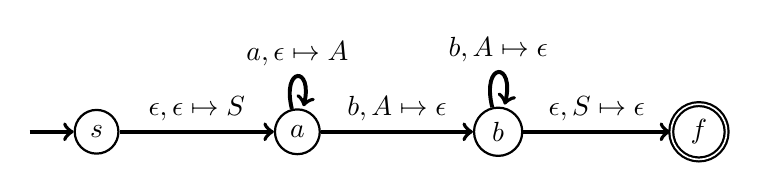
\begin{tikzpicture}[xscale=0.85,baseline={([yshift=-2ex]current bounding box.north)}]
% \draw[help lines] (0,0) grid (7,2);
\node (s) [circle,draw=black,thick] at (0,0) {$s$};
\node (a) [circle,draw=black,thick] at (3,0) {$a$};
\node (b) [circle,draw=black,thick] at (6,0) {$b$};
\node (f) [circle,draw=black,thick,double] at (9,0) {$f$};
% \node (e) [circle,draw=black,thick] at (4.5,-1) {$e$};
%
\path[->,line width=0.5mm](-1,0) edge (s);
\path[->,line width=0.5mm](s) edge node[above] {$\epsilon,\epsilon\mapsto\Snterm{S}$} (a);
\path[->,line width=0.5mm](a) edge [loop above] node[above] {$\Sterm{a},\epsilon\mapsto\Snterm{A}$} (a);
\path[->,line width=0.5mm](a) edge node[above] {$\Sterm{b},\Snterm{A}\mapsto\epsilon$} (b);
\path[->,line width=0.5mm](b) edge [loop above] node[above] {$\Sterm{b},\Snterm{A}\mapsto\epsilon$} (b);
\path[->,line width=0.5mm](b) edge node[above] {$\epsilon,\Snterm{S}\mapsto\epsilon$} (f);

% \path[->,line width=0.5mm,bend right](s) edge node[below] {$\epsilon,\epsilon\mapsto\Snterm{S}$} (e);
% \path[->,line width=0.5mm,bend right](e) edge node[below] {$\epsilon,\Snterm{S}\mapsto\epsilon$} (f);
\end{tikzpicture}}\bigskip

Dieser PDA erfüllt die Anforderungen aus dem Beweis.\\[1ex]
Als Grammatik ergibt sich:
% 
\begin{align*}
\Sntermsub{V}{s,f} & \to \epsilon\Sntermsub{V}{a,b}\epsilon\\
\Sntermsub{V}{a,b} & \to \Sterm{a}\Sntermsub{V}{a,b}\Sterm{b}\mid \Sterm{a}\Sntermsub{V}{a,a}\Sterm{b}\\
\Sntermsub{V}{a,a} & \to \epsilon \qquad \Sntermsub{V}{b,b}\to \epsilon\qquad \Sntermsub{V}{s,s}\to \epsilon\qquad \Sntermsub{V}{f,f}\to \epsilon \\
\Sntermsub{V}{a,a} & \to\Sntermsub{V}{a,a}\Sntermsub{V}{a,a}\mid\Sntermsub{V}{a,b}\Sntermsub{V}{b,a}\mid\Sntermsub{V}{a,s}\Sntermsub{V}{s,a}\mid\Sntermsub{V}{a,f}\Sntermsub{V}{f,a}\qquad
\Sntermsub{V}{a,b}\to\ldots\qquad\ldots
\end{align*}

\textcolor{devilscss}{(nicht alle dieser Regeln werden wirklich benötigt)}

\end{frame}

% \begin{frame}\frametitle{Ausdrucksstärke von PDAs}
% 
% Damit haben wir beide Richtungen des wichtigsten Ergebnisses dieser Vorlesung gezeigt:
% \medskip
% 
% \theobox{Satz: Eine Sprache ist genau dann kontextfrei wenn sie von einem PDA akzeptiert wird.}\pause\bigskip
% % \theobox{Satz: Eine Sprache $\Slang{L}$ ist kontextfrei genau dann wenn es einen PDA $\Smach{M}$ mit 
% % $\Slang{L}(\Smach{M})=\Slang{L}$ gibt.}\pause\bigskip
% 
% Der Beweis erfolgt in zwei Schritten:
% \begin{enumerate}[(1)]
% \item Umwandlung PDA $\leadsto$ Typ-2-Grammatik
% \item Umwandlung Typ-2-Grammatik $\leadsto$ PDA
% \end{enumerate}
% 
% \end{frame}

% \begin{frame}\frametitle{Lehrevaluation}
% 
% % \huge
% 
% \begin{center}
% 15min zum Ausfüllen der Fragebögen
% \end{center}
% 
% \end{frame}

\sectionSlide{Deterministische Kellerautomaten}

\begin{frame}\frametitle{Deterministische Kellerautomaten?}

Es gibt verschiedene Quellen für Nichtdeterminismus bei PDAs\pause:
\begin{itemize}
\item Übergangsfunktion liefert eine Menge möglicher Übergänge\pause
\item Mehrere mögliche Startzustände\pause
\item $\epsilon$-Übergänge in Eingabe und Keller\medskip

\examplebox{\emph{Beispiel:}
Angenommen es gilt $\delta(q,\epsilon,\Snterm{A})=\{\tuple{p,\Snterm{B}}\}$ und
$\delta(q,\Sterm{a},\epsilon)=\{\tuple{r,\Snterm{C}}\}$. Dann gibt es mehrere mögliche
Übergänge, wenn in Zustand $q$ das Symbol \Sterm{a} gelesen wird und \Snterm{A} auf dem
Keller liegt. Und das obwohl die Übergangsfunktion nur einelementige Mengen liefert.
}
\end{itemize}

Deterministische Kellerautomaten müssen eingeschränkt werden, ohne 
$\epsilon$-Übergänge ganz zu verbieten (ganz ohne $\epsilon$-Übergänge sind PDAs zu schwach)

\end{frame}

\begin{frame}\frametitle{Deterministische Kellerautomaten}

\defbox{Ein \redalert{deterministischer Kellerautomat} (international: "`\alert{DPDA}"') 
\Smach{M} ist ein Tupel $\Smach{M}=\tuple{Q,\Sigma,\Gamma,\delta,q_0,F}$ mit
den folgenden Bestandteilen:
\begin{itemize}
\item $Q$: endliche Menge von \redalert{Zuständen}
\item $\Sigma$: \redalert{Eingabealphabet}
\item $\Gamma$: \redalert{Kelleralphabet}
\item $\delta$: \redalert{Übergangsfunktion}, eine partielle Funktion\\[1ex]
\narrowcentering{$Q\times\Sigma_\epsilon\times\Gamma_\epsilon \to Q\times\Gamma_\epsilon$,}\\[1ex]
~~~~so dass für alle $q\in Q$, $\Sterm{a}\in\Sigma$ und $\Snterm{A}\in\Gamma$\\
~~~~jeweils nur eines der folgenden definiert ist:\\[1ex]
\narrowcentering{$\delta(q,\Sterm{a},\Snterm{A})$\hfill$\delta(q,\Sterm{a},\epsilon)$\hfill$\delta(q,\epsilon,\Snterm{A})$\hfill$\delta(q,\epsilon,\epsilon)$}
\item $q_0$: ein \redalert{Startzustand} $q_0\in Q$
\item $F$: Menge von \redalert{Endzuständen} $F\subseteq Q$
\end{itemize}

}

\end{frame}

\begin{frame}\frametitle{Beispiele}

Dieser Automat ist ein DPDA:\medskip

\narrowcentering{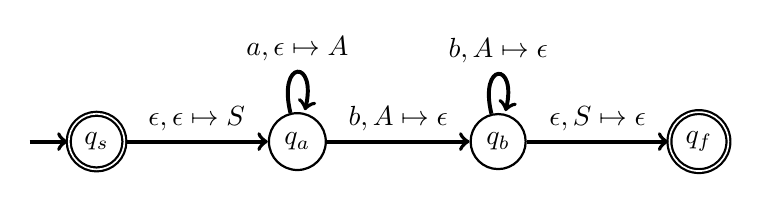
\begin{tikzpicture}[xscale=0.85,baseline={([yshift=-2ex]current bounding box.north)}]
% \draw[help lines] (0,0) grid (7,2);
\node (s) [circle,draw=black,thick,double] at (0,0) {$q_s$};
\node (a) [circle,draw=black,thick] at (3,0) {$q_a$};
\node (b) [circle,draw=black,thick] at (6,0) {$q_b$};
\node (f) [circle,draw=black,thick,double] at (9,0) {$q_f$};
%
\path[->,line width=0.5mm](-1,0) edge (s);
\path[->,line width=0.5mm](s) edge node[above] {$\epsilon,\epsilon\mapsto\Snterm{S}$} (a);
\path[->,line width=0.5mm](a) edge [loop above] node[above] {$\Sterm{a},\epsilon\mapsto\Snterm{A}$} (a);
\path[->,line width=0.5mm](a) edge node[above] {$\Sterm{b},\Snterm{A}\mapsto\epsilon$} (b);
\path[->,line width=0.5mm](b) edge [loop above] node[above] {$\Sterm{b},\Snterm{A}\mapsto\epsilon$} (b);
\path[->,line width=0.5mm](b) edge node[above] {$\epsilon,\Snterm{S}\mapsto\epsilon$} (f);
\end{tikzpicture}}

\bigskip\bigskip

Dieser Automat ist \redalert{kein} DPDA:\medskip

\narrowcentering{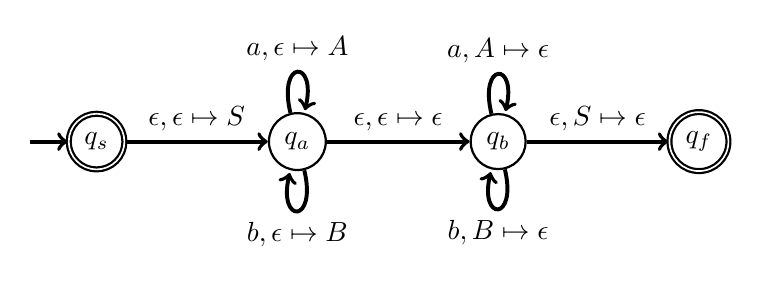
\begin{tikzpicture}[xscale=0.85,baseline={([yshift=-2ex]current bounding box.north)}]
% \draw[help lines] (0,0) grid (7,2);
\node (s) [circle,draw=black,thick,double] at (0,0) {$q_s$};
\node (a) [circle,draw=black,thick] at (3,0) {$q_a$};
\node (b) [circle,draw=black,thick] at (6,0) {$q_b$};
\node (f) [circle,draw=black,thick,double] at (9,0) {$q_f$};
%
\path[->,line width=0.5mm](-1,0) edge (s);
\path[->,line width=0.5mm](s) edge node[above] {$\epsilon,\epsilon\mapsto\Snterm{S}$} (a);
\path[->,line width=0.5mm](a) edge [loop above] node[above] {$\Sterm{a},\epsilon\mapsto\Snterm{A}$} (a);
\path[->,line width=0.5mm](a) edge [loop below] node[below] {$\Sterm{b},\epsilon\mapsto\Snterm{B}$} (a);
%
% \path[->,line width=0.5mm,bend left=20](a) edge node[above] {$\Sterm{a},\Snterm{A}\mapsto\epsilon$} (b);
% \path[->,line width=0.5mm,bend right=20](a) edge node[below] {$\Sterm{b},\Snterm{B}\mapsto\epsilon$} (b);
\path[->,line width=0.5mm](a) edge node[above] {$\epsilon,\epsilon\mapsto\epsilon$} (b);
\path[->,line width=0.5mm](b) edge [loop above] node[above] {$\Sterm{a},\Snterm{A}\mapsto\epsilon$} (b);
\path[->,line width=0.5mm](b) edge [loop below] node[below] {$\Sterm{b},\Snterm{B}\mapsto\epsilon$} (b);
\path[->,line width=0.5mm](b) edge node[above] {$\epsilon,\Snterm{S}\mapsto\epsilon$} (f);
\end{tikzpicture}}

\end{frame}

\begin{frame}\frametitle{Deterministische kontextfreie Sprachen}

DPDAs führen zu einer eigenen Sprachklasse:

\defbox{Eine Sprache ist \redalert{deterministisch kontextfrei} wenn sie durch einen deterministischen Kellerautomaten
akzeptiert wird.}

Offensichtlich ist jede deterministisch kontextfreie Sprache auch kontextfrei (DPDAs können als PDAs gesehen werden).
\medskip\pause

Im Gegensatz zur Situation bei DFAs und NFAs gilt die Umkehrung dieser Aussage nicht:\medskip

\theobox{\emph{Satz:} Die deterministisch kontextfreien Sprachen bilden eine echte Untermenge der kontextfreien Sprachen.\\
Es gibt also kontextfreie Sprachen, die nicht deterministisch sind.}

\end{frame}

\begin{frame}\frametitle{Abschluss unter Komplement}

Der Unterschied zu allgemeinen kontextfreien Sprachen zeigt sich gut am folgenden Ergebnis:

\theobox{\emph{Satz:} Die Klasse der deterministisch kontextfreien Sprachen ist unter Komplement abgeschlossen.}\medskip

\emph{Beweisidee: } Wie bei DFAs kann man auch bei DPDAs die akzeptierenden und nichtakzeptierenden Zustände 
vertauschen.\\
Mehrere technische Komplikationen machen den Beweis etwas aufwändiger:

{\tiny
\begin{itemize}
\item Ein DPDA kann ein Wort auf zwei Arten nicht akzeptieren: (1) nach dem Lesen der Eingabe ist der Automat
nicht in einem Endzustand; (2) die Eingabe wird nie ganz gelesen, z.B. weil der Automat in eine Endlosschleife von 
$\epsilon$-Übergängen gerät. Man muss Grund (2) ausschalten.
\item Ein Lauf
könnte mit einer Folge von $\epsilon$-Übergängen enden, die akzeptierende und nichtakzeptierende Zustände enthält. In diesem Fall führt Austausch der Endzustände nicht zum gewünschten Ergebnis. Man
muss sicherstellen, dass grundsätzlich (vor und nach der Komplementierung) nur der erste Zustand in einer Folge von
$\epsilon$-Übergängen akzeptieren darf.
\end{itemize}}
{\tiny (vollständiger Beweis siehe Sipser, Abschnitt 2.4)}\qed

\end{frame}

\begin{frame}\frametitle{Nichtdeterministische kontextfreie Sprachen}

Eine kontextfreie Sprache, deren Komplement nicht kontextfrei ist, kann demnach nicht deterministisch kontextfrei sein.

\examplebox{Beispiel: In Vorlesung 14 haben wir die Sprachen $\Slangsub{L}{1}=\{\Sterm{a}^i\Sterm{b}^i\Sterm{c}^k\mid i\geq 0, k\geq 0\}$ und $\Slangsub{L}{2}=\{\Sterm{a}^i\Sterm{b}^k\Sterm{c}^k\mid i\geq 0, k\geq 0\}$ betrachtet und erkannt,
dass die Sprache 
\[
\overline{\Slangsub{L}{1}}\cup\overline{\Slangsub{L}{2}}=\{\Sterm{a}^i\Sterm{b}^j\Sterm{c}^k\mid i\neq j \text{ oder }j\neq k\}\,\cup\,
\big(\{\Sterm{a},\Sterm{b},\Sterm{c}\}^*\circ\{\Sterm{ba},\Sterm{ca},\Sterm{cb}\}\circ\{\Sterm{a},\Sterm{b},\Sterm{c}\}^*\big)
% \Slang{L}()
\]
kontextfrei ist, aber ihr Komplement nicht. Diese Sprache ist demnach nicht deterministisch kontextfrei.}

Das beweist im Wesentlichen die Behauptung, dass die deterministisch kontextfreien Sprachen eine echte Untermenge der
kontextfreien sind.\medskip\pause

Es gibt noch viele andere nichtdeterministische Sprachen, z.B.:

\examplebox{\emph{Beispiel:} Die Sprache $\{w w^r\mid w\in\{\Sterm{a},\Sterm{b}\}^*\}$ der Palindrome gerader Länge (ohne Markierung in der Mitte) ist kontextfrei aber nicht deterministisch. \\(Ohne Beweis; siehe z.B. Skript Franz Baader)}

\end{frame}


% \begin{frame}\frametitle{Determinismus vs. Mehrdeutigkeit}
% \end{frame}

\begin{frame}\frametitle{Zusammenfassung und Ausblick}

% PDAs erlauben \redalert{verschiedene äquivalente Definitionen}
% \bigskip

PDAs erkennen \redalert{genau die kontextfreien Sprachen}:
\begin{itemize}
\item PDA $\leadsto$ Typ-2-Grammatik durch Simulation von Linksableitungen
\item Typ-2-Grammatik $\leadsto$ PDA durch rekursive Erzeugung der Sprachen $\Slangsub{L}{q,r}$
\end{itemize}
\bigskip

\redalert{Deterministische Kellerautomaten} (DPDAs) erkennen nur eine echte Untermenge der kontextfreien Sprachen.
\bigskip

\anybox{yellow}{
Offene Fragen:
\begin{itemize}
\item Wozu sind deterministische kontextfreie Sprachen gut?
\item Welche Probleme auf CFGs kann man lösen?
\item Was gibt es zu Typ 1 und Typ 0 zu sagen?
\end{itemize}
}

\end{frame}


\end{document}
